\section{Background}
\label{sec:background}

\subsection{RDMA}

\begin{figure*}[t]
    \centering
    \begin{subfigure}{0.3\linewidth}
        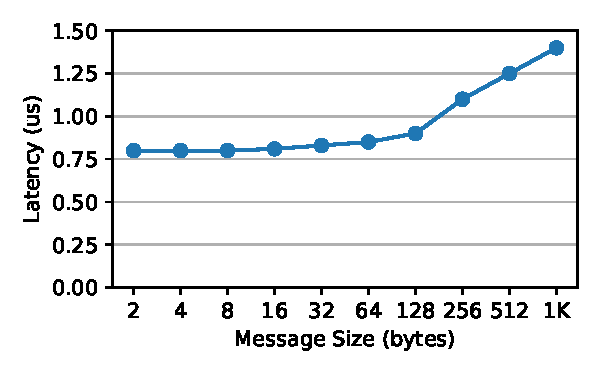
\includegraphics[width=0.99\linewidth]{fig/rdma_latency.pdf}
        % \label{fig:rdma_latency}
        % \caption{}
    \end{subfigure}
    \begin{subfigure}{0.3\linewidth}
        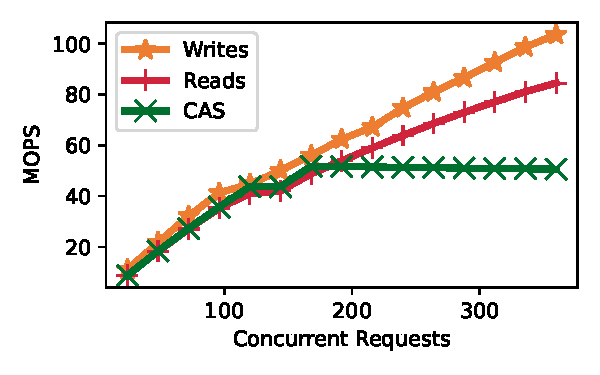
\includegraphics[width=0.99\linewidth]{fig/rdma_concur.pdf}
        % \label{fig:optimistic_failures}
        % \caption{}
    \end{subfigure}
    \begin{subfigure}{0.3\linewidth}
        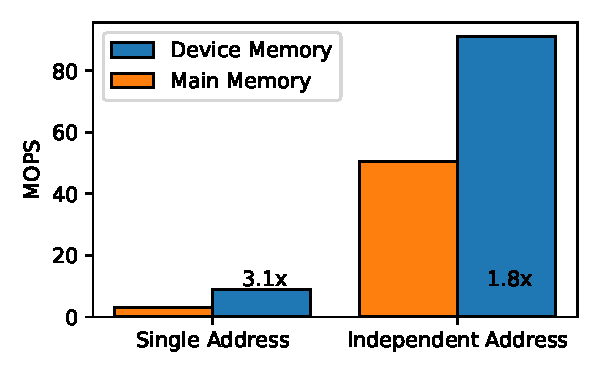
\includegraphics[width=0.99\linewidth]{fig/rdma_cas_throughput.pdf}
        % \label{fig:optimistic_failures}
        % \caption{}
    \end{subfigure}
    \vspace{-1em}
    \caption{
    \textbf{(a)} CX5 RDMA latency vs message size~\cite{rdma-latency}
    \textbf{(b)} RDMA operation scalability
    \textbf{(c)} Compare and swap performance. Device memory vs main memory.
    }
    \label{fig:rdma-benchmarks}
\end{figure*}


RDMA NIC bandwidth has increased disproportionately to
latency in the last decade leading to interesting design
tradeoffs. CX7 NICs have 10$\times$ the bandwidth of CX3's
but their intra-rack RTT has only shrunk by 1.5$\times$.
Figure~\ref{fig:rdma-benchmarks}(a) shows NIC-to-NIC round
trips times on CX5s for variable sized writes. All writes up
to 128 bytes have comparable latencies and writes must
exceed 1KB before the latency of a single large packet
exceeds two round trips of smaller writes. \textbf{If there
is surplus bandwidth a single large message can have much
lower latency than two dependent smaller messages.}

RDMA is an enabling technology for memory disaggregation. It
allows client machines to directly access the memory of a
remote server with one-sided operations like read, write and
atomic update without the involvement of a remote
CPU~\cite{infiniband-spec}.  
%%
Atomic operations such as compare-and-swap (CAS) are
essential for implementing locks or opportunistic
concurrency. Atomics are limited to 64 bit operations and
bottleneck at lower ops/s than reads and writes because they
block requests on data dependent addresses while waiting on
PCIe round trips~\cite{design-guidelines,sherman}.
Figure~\ref{fig:rdma-benchmarks}(b) shows the scalability of
these operations on CX5 NICs for 64 bit operations.
%%
Vendors have provided some workarounds for atomic
bottlenecks by adding device memory and masked atomic
operations. CX series NICs have a 256KB region of on-NIC
RDMAable memory. Atomics to this region avoid the round trip
and execute with lower latency and up to 3x higher
throughput~\cite{device-memory}(Figure~\ref{fig:rdma-benchmarks}(c)).
Masked compare and swap enables each bit to be set
independently thus enabling higher density locks while
reducing contention~\cite{rdma-masked-cas}. While multi-CAS
is not supported these features have been demonstrated to
enable fast dense lock tables~\cite{sherman}.


\subsection{RDMA Key-Value Stores}

%% %Describe existing key value stores relation to rdma and
%serialization %
Many non-disaggregated key-value stores have used RDMA to
accelerate their
performance~\cite{farm,memc3,erpc,herd,faast,mica,pilaf,cell,storm}.
%%
These systems strike a careful balance between directly
accessing memory with client side RDMA and serializing
requests with a server side CPU.
%%
Cuckoo and Hopscotch hashes have flourished in this space
because clients can locally calculate the location of keys
and perform lockless $O(1)$ reads with
RDMA~\cite{hopscotch,farm,pilaf,cuckoo}.
%%
Disaggregated key-value in contrast assume that a memory
server cannot provide serialization and orchestrate their
writes solely using
clients~\cite{rolex,fusee,clover,sherman,ford,race}. With
the exception of Sherman~\cite{sherman} these systems use
systems commit writes optimistically using 64 bit RDMA CAS. 
%%
Opportunistic writes have the advantage that updates are
atomically visible, no critical sections exist, and client
failures do not leave the table in an inconsistent state.
Unfortunately CAS based opportunistic writes perform poorly
under contention leading to high tail latencies
~\cite{clover}. Additionally RDMA CAS does not scale
well~\cite{design-guidelines}(Figure~\ref{fig:rdma-benchmarks}(b)),
and their small word width and lack of multi-CAS support
constrain the size and types of updates they can perform.

CAS width in particular effects system design because
key-value pairs can rarely fit into 64 bits, indexes updated
with CAS must reference keys values indirectly with a
pointer. At minimum resolving a remote pointer requires an
additional round trip for every read~\cite{race,clover}.
%%
As we will show in the following section data structures
like cuckoo and hopscotch hashes are difficult implement with
optimistic CAS updates because they require multiple updates
to execute atomically.


\subsection{Cuckoo Hashing} 
\label{sec:cuckoo-back}
Cuckoo hashing uses two independent hash functions to assign
keys a primary and secondary table location. When a key is
inserted if its primary location is occupied the existing
key is evicted to its alternative location. If the eviction
causes another collision the process iterates until an open
location is found. The path of evictions is known as
a~\textit{cuckoo path}. Cuckoo hashes use associative rows
to improve their maximum fill factors. In associative hashes
multiple clients can be chosen as eviction candidates and
breadth-first-search (BFS) has been shown to minimize both
cuckoo path length and critical section time~\cite{memc3,
cuckoo-improvements}.  While insertions require large
critical sections to perform search and execute updates
along the cuckoo path reads are executed in constant time by
reading both of a keys buckets~\cite{pilaf}.

%%now I want to explain why cuckoo hashing and disaggregation don't work well together.

Lockless $O(1)$ reads make Cuckoo hashing a desireable
candidate for a disaggregated index. However, long
unpredictable cuckoo paths and RDMA CAS limitations make
performing insertions without locks difficult in the
disaggregated setting. We designed an RDMA based cuckoo hash
to illustrate the difficulties of performing opportunistic
insertions. On inserts this system makes a sequence of reads
to calculate a valid cuckoo path and then itteratitivly
issues CAS operations to swap value along the path. If any
value on the path is concurrently modified by another client
the insertions will fail and must restart.
Figure~\ref{fig:cuckoo-problems}(a) shows how the failure
rate of insertions filling a table from 80-90\% full.

\textbf{Hopscotch Hashing} also enables fast reads by
localizing entries to a bounded range of addresses and we
considered using it as our core data structure. We believe
that although hopscotch hashing can likely be disaggregated
efficiently it is less straightforward than cuckoo hashing
for the following reasons:
%%
First, cuckoo insertions update one location per moved key while
hopscotch requires two. Hopscotch hashes keep a bitmask of
collisions per bucket which must also be updated when an
entry is relocated. Reno, a heavily one-sided RDMA hopscotch
hash, uses one sided atomics to sloppily update the bitmask
but requires a server side CPU to fix the bitmasks whenever
concurrent inserts execute~\cite{reno}. Both Farm and Reno
avoid ever executing long hopscotch chains because of their
execution time and complexity~\cite{farm,reno}.
%%
Second, an entries location in a cuckoo hash is easier to
predict than in hopscotch hashing which simplifies locking.
Cuckoo keys inhabit exactly one of two locations so locks
are predictable, conversely hopscotch locations occur on a
range so a locking strategy must lock the entire range
conservatively. Because each lock acquisition is expensive
this increases the fundamental difficulty of disaggregation
a hopscotch hash.